\documentclass[a4paper,fleqn]{cas-dc}
\usepackage{graphicx}
\usepackage{color}
\usepackage{import}
\usepackage[numbers,sort&compress]{natbib}
\usepackage{amsmath}
\usepackage{amssymb}
\usepackage{booktabs}
\usepackage{tikz}
\usepackage{pgfplots}
\pgfplotsset{compat=1.18}
\usetikzlibrary{arrows.meta,positioning}

% Figures use this preamble macro; precompiled figures keep its rendering.
\newcommand{\Cycle}{k}

\begin{document}
\shorttitle{Flat Elsevier submission demo}
\shortauthors{J. Doe et~al.}

\title[mode = title]{A Demonstration Manuscript for Flat Elsevier Editorial Manager Submissions}

\author[1]{Jane Doe}
\cormark[1]
\ead{jane.doe@example.org}

\author[1]{John Roe}
\ead{john.roe@example.org}

\affiliation[1]{organization={Example Institute}, city={Example City}, country={Exampleland}}

\cortext[cor1]{Corresponding author}

\begin{abstract}
This dummy manuscript exercises the submission pipeline. Its sources live in subfolders and contain a TikZ diagram, a PGFPlots figure that reads CSV data, and an SVG drawing exported from Inkscape as PDF with a \LaTeX{} text overlay. The pipeline copies everything into one flat folder and can render each figure as a standalone PDF.
\end{abstract}

\begin{highlights}
\item Subfolder sources are flattened into a single upload folder.
\item TikZ, PGFPlots and Inkscape figures are rendered as PDFs in context.
\item The flat submission compiles locally before upload.
\end{highlights}

\begin{keywords}
\LaTeX{} \sep Editorial Manager \sep TikZ \sep Inkscape
\end{keywords}

\maketitle

\section{Introduction}

Editorial Manager expects a flat set of source files, whereas manuscripts are usually organized in folders~\citep{knuth1986texbook}. Figure~\ref{fig:workflow} shows the export steps as a TikZ diagram~\citep{tantau2023tikz}.

\begin{figure}[t]
\centering
\resizebox{\columnwidth}{!}{% TikZ diagram. Exported as workflow.tex; --precompile renders it as a PDF.
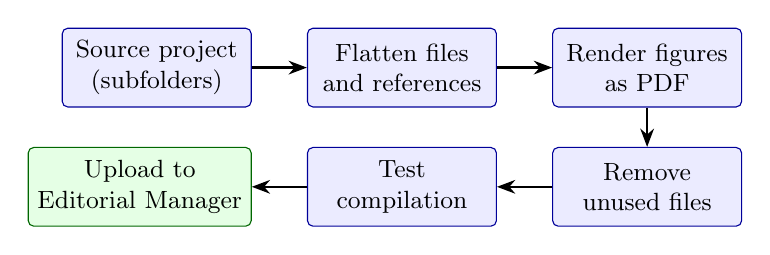
\begin{tikzpicture}[
  node distance=5mm and 7mm,
  stage/.style={draw=blue!60!black, fill=blue!8, rounded corners=2pt,
    minimum width=24mm, minimum height=10mm, align=center, font=\small},
  flow/.style={-Stealth, thick},
]
  \node[stage] (source) {Source project\\(subfolders)};
  \node[stage, right=of source] (flatten) {Flatten files\\and references};
  \node[stage, right=of flatten] (render) {Render figures\\as PDF};
  \node[stage, below=of render] (prune) {Remove\\unused files};
  \node[stage, left=of prune] (test) {Test\\compilation};
  \node[stage, left=of test, fill=green!10, draw=green!40!black] (upload) {Upload to\\Editorial Manager};

  \draw[flow] (source) -- (flatten);
  \draw[flow] (flatten) -- (render);
  \draw[flow] (render) -- (prune);
  \draw[flow] (prune) -- (test);
  \draw[flow] (test) -- (upload);
\end{tikzpicture}
}
\caption{Export workflow drawn with TikZ.}
\label{fig:workflow}
\end{figure}

\section{Figures with external files}

Figure~\ref{fig:results} is a PGFPlots~\citep{feuersanger2021pgfplots} figure that reads its data from a CSV file. The extensionless input below is resolved to \texttt{results.tex} in the flat export, and the CSV path inside the figure is rewritten as well.

\begin{figure}[t]
\centering
% PGFPlots figure with external CSV data. The CSV path is rewritten when the
% project is flattened; --precompile renders the plot and drops the CSV.
\begin{tikzpicture}
  \begin{axis}[
    width=\columnwidth, height=4.5cm,
    xlabel={Cycle $\Cycle$}, ylabel={Quality index},
    xmin=0, xmax=14, ymin=0.2, ymax=1.15,
    grid=major, legend pos=south east, legend cell align=left,
  ]
    \addplot[blue, thick, mark=*, mark size=1pt] table[x=cycle, y=measured, col sep=comma] {./figure/results/results_data.csv};
    \addlegendentry{Measured}
    \addplot[black, dashed] table[x=cycle, y=reference, col sep=comma] {./figure/results/results_data.csv};
    \addlegendentry{Reference}
  \end{axis}
\end{tikzpicture}

\caption{Convergence over cycles $\Cycle$, plotted with PGFPlots from \texttt{results\_data.csv}.}
\label{fig:results}
\end{figure}

Figure~\ref{fig:setup} was drawn in \texttt{setup.svg} and exported by Inkscape as \texttt{setup.pdf} with the text overlay \texttt{setup.pdf\_tex}. Its labels are typeset by \LaTeX{} and use the manuscript's \verb|\Cycle| macro.

\begin{figure}[t]
\centering
\def\svgwidth{\columnwidth}
\import{./figure/setup/}{setup.pdf_tex}
\caption{Closed-loop setup drawn in Inkscape and exported as PDF with a \LaTeX{} overlay.}
\label{fig:setup}
\end{figure}

\section{Conclusion}

After \verb|flatten_submission.py --precompile|, the three figures above are included as \texttt{figure-01-workflow.pdf}, \texttt{figure-02-results.pdf} and \texttt{figure-03-setup.pdf}, and their TikZ, CSV, SVG and overlay sources are no longer part of the upload.

\bibliographystyle{cas-model2-names}
\bibliography{references}

\end{document}
